"present papers from the coding perspective so that reproducibility and replication of results in the Machine Learning community becomes easier"


Need some information (and reference(s)) about IRBs and human subjects research?

Re-identification attacks - should we include brief description about this? Some references: 
* El Emam K, Jonker E, Arbuckle L, Malin B. A systematic review of re-identification attacks on health data. PLoS ONE 2011;6(12) [e28071, 12].
* Sweeney L. k-anonymity: a model for protecting privacy. Ijufks 2002;10:557–70.

\section{Introduction}

Reproducing machine learning results in the field of health care is challenging. Historically, many published research articles do not make code nor data available which limits the ability of other researchers to validate or reproduce results. While some high impact journals such as the Nature Research journal family have adopted policies to promote software and data sharing \cite{natmethods}, not all journals and locations where machine learning methods are published have such policies. Despite a growing trend toward code and data sharing policies, there are additional difficulties in sharing health care data due to legal requirements. 

 In the U.S., the primary law affecting health data privacy is the Health Insurance Portability and Accountability Act (HIPAA) \cite{hippapro}. Additionally, organizations desiring to perform biomedical and social, behavioral, and educational research are subject to Common Rule (45 CFR 46, Subpart A) and/or the U.S. Food and Drug Administration’s regulations (21 CFR 50 and 56). Furthermore, the Common Rule established Institutional Review Boards which are responsible and the institutional level of safe guarding human subjects in any research; similar layers of laws and legal controls exist in other countries. Due to the many constraints in place, even appropriate and routine requests to access data can take a significant amount of effort and time. Importantly, only the approved group or individual can access data; it cannot be shared in original form or used for other purposes, so secondary, educational or other key data use cases are left unmet.
 
 As machine learning results are highly data dependent, the barriers around sharing health data make it difficult or impossible for others to verify or reproduce results with novel machine learning methods in the health care domain (? cite recent non-reproducible examples such as Google FHIR, others?). In order to resolve the problem of data sharing, various methods for data synthesis and de-identification have been developed in other data domains that have been applied to health care. The use of privacy preserving techniques as methods to safely share health care or other data have a history of re-identification risk as detailed by Sweeney \cite{sweeney_2002}. Alternative techniques of synthetic data have been used to avoid the potential problem of re-identification. One early example by Gray et al. \cite{gray_quickly_1994} used pseudo-random generation techniques to populate large databases with synthetic data for performance evaluation. Subsequent advances in techniques have generated more realistic data based on observed and publicly reported statistics, such as with the Synthea system \cite{walonoski_synthea:_2018}, that generates an entire outpatient Electronic Health Record (EHR) based on population statistics. 
 
 While advances in both de-identification and synthesis of data have been impressive, still more progress needs to be made. Techniques such as Synthea that generate an entire EHR require significant computational power and model development of every disease state desired and may not have the level of specificity as found in an actual EHR due to rare or complex conditions. Other techniques based on actual health data such as described by Gal et al. \cite{gal_data_2014} provide for the complexities found in real health data by building off of the condensation algorithm \cite{aggarwal_static_2008} though use of k-means clustering, Principle Component Analysis, and independent data generation pipelines based on a specific outcome variable. While the method as depicted by Gal results in a use case specific synthetic data set, the manual intervention required to develop a synthetic data requires an ongoing effort between the data source and researchers needing access to data. In this paper we propose a method that allows the user of the data to identify what attributes they are interested in, does not require manual intervention or generation of synthetic data, and is modular so that as new techniques are developed the system could be updated to take advantage of them.
 
 \section{Reproducibility}
 %Good discussion of what reproducibility vs replicability means
 %http://languagelog.ldc.upenn.edu/nll/?p=21956
 Over the past 18 years, there has been several significant papers clarifying the definition and importance of reproducibility along with the closely related term replicability. Leek and Peng have defined reproducibility as the "ability to recompute data analytic results given an observed dataset and knowledge of the data analysis pipeline," and replicability as "the chance that an independent experiment targeting the same scientific question will produce a consistent result" \cite{leek_opinion_2015}; others such as Drummond use the terms in a reverse fashion \cite{drummond_replicability_2009}. Despite the semantic disagreement, both groups agree that an independent experiment with confirmatory results is the strongest support of any experiment. One early influential paper on the topic of reproducibility in scientific computing details key factors in reproducibility as having: data, input parameters, documentation, software code, and an environment capable of running the provided software code; items that cannot easily nor clearly be communicated by paper \cite{schwab_making_2000}. Reproducibility should be treated as a minimum required standard that all published research should meet \cite{peng_reproducible_2006}. Specifically in the context of machine learning, this means including details to a level someone else could create the same environment including hardware configuration and run times, data used for all experiments, source code, documentation on data and how to run/configure software, and tests that verify the software runs correctly. The last item is important but often overlooked - unit tests can show how a researcher validated their code was giving expected results which can often lead to insights not normally communicated in a results section of a journal article. Once a result can be reproduced, new researchers can then build upon the methods, gather new data for testing/validation, or discover alternative methods to replicate a result.
 
 techniques for privacy protection:
 * De-identifcation
   * removal of known unique identifiers
   * Data summarization to prevent individual identification
   * Problem: "Although these techniques support privacy protected data publishing without synthesis, the degree of privacy protection they provide depends on the background knowledge of adversaries."
 * Synthesis - Generating data based on some statistical model; "...the process of creating artificial data that can be used to serve some key purposes of real data."
 
 
 % Some information about minimum group size
 %* Minimum group/result set size depends on several factors such as re-identification risk, number of attributes available (see picture at end)
 %* Individual states have adopted minimum group size reporting rules, with the minimum number of students ranging from 5 to 30 and a modal category of 10 (used by 39 states) https://nces.ed.gov/pubs2011/2011603.pdf
 %* 62 https://nces.ed.gov/nationsreportcard/tdw/analysis/summary_rules_minimum.aspx
 %* 30; describes techniques to determine size - https://nces.ed.gov/pubs2017/2017147.pdf
 
 % removed since we never got SGF working
 \begin{table}
  \caption{Kung Faux Pandas data synthesis methods}
  \label{included-methods}
  \centering
  \begin{tabular}{p{12em} l p{14em}}
    \toprule
    Method                                 & Source                    & Notes \\
    \midrule
    Kernel Density Estimator               & scipy.stats.gaussian\_kde & Inter-related ordinal and ratio data\\
    DataSynthesizer                        & Ping et al.               & Bayesian modeling of column relationships\\
    Synthetic dataset Generation Framework & Bindschaedler et al.      & "Plausible Deniability" probabilistic modeling\\
    \bottomrule
  \end{tabular}
\end{table}


\begin{wrapfigure}[15]{r}{0.5\textwidth}%optionally place [15] after {wrapfigure} to control how many lines to wrap around figure
  \centering
  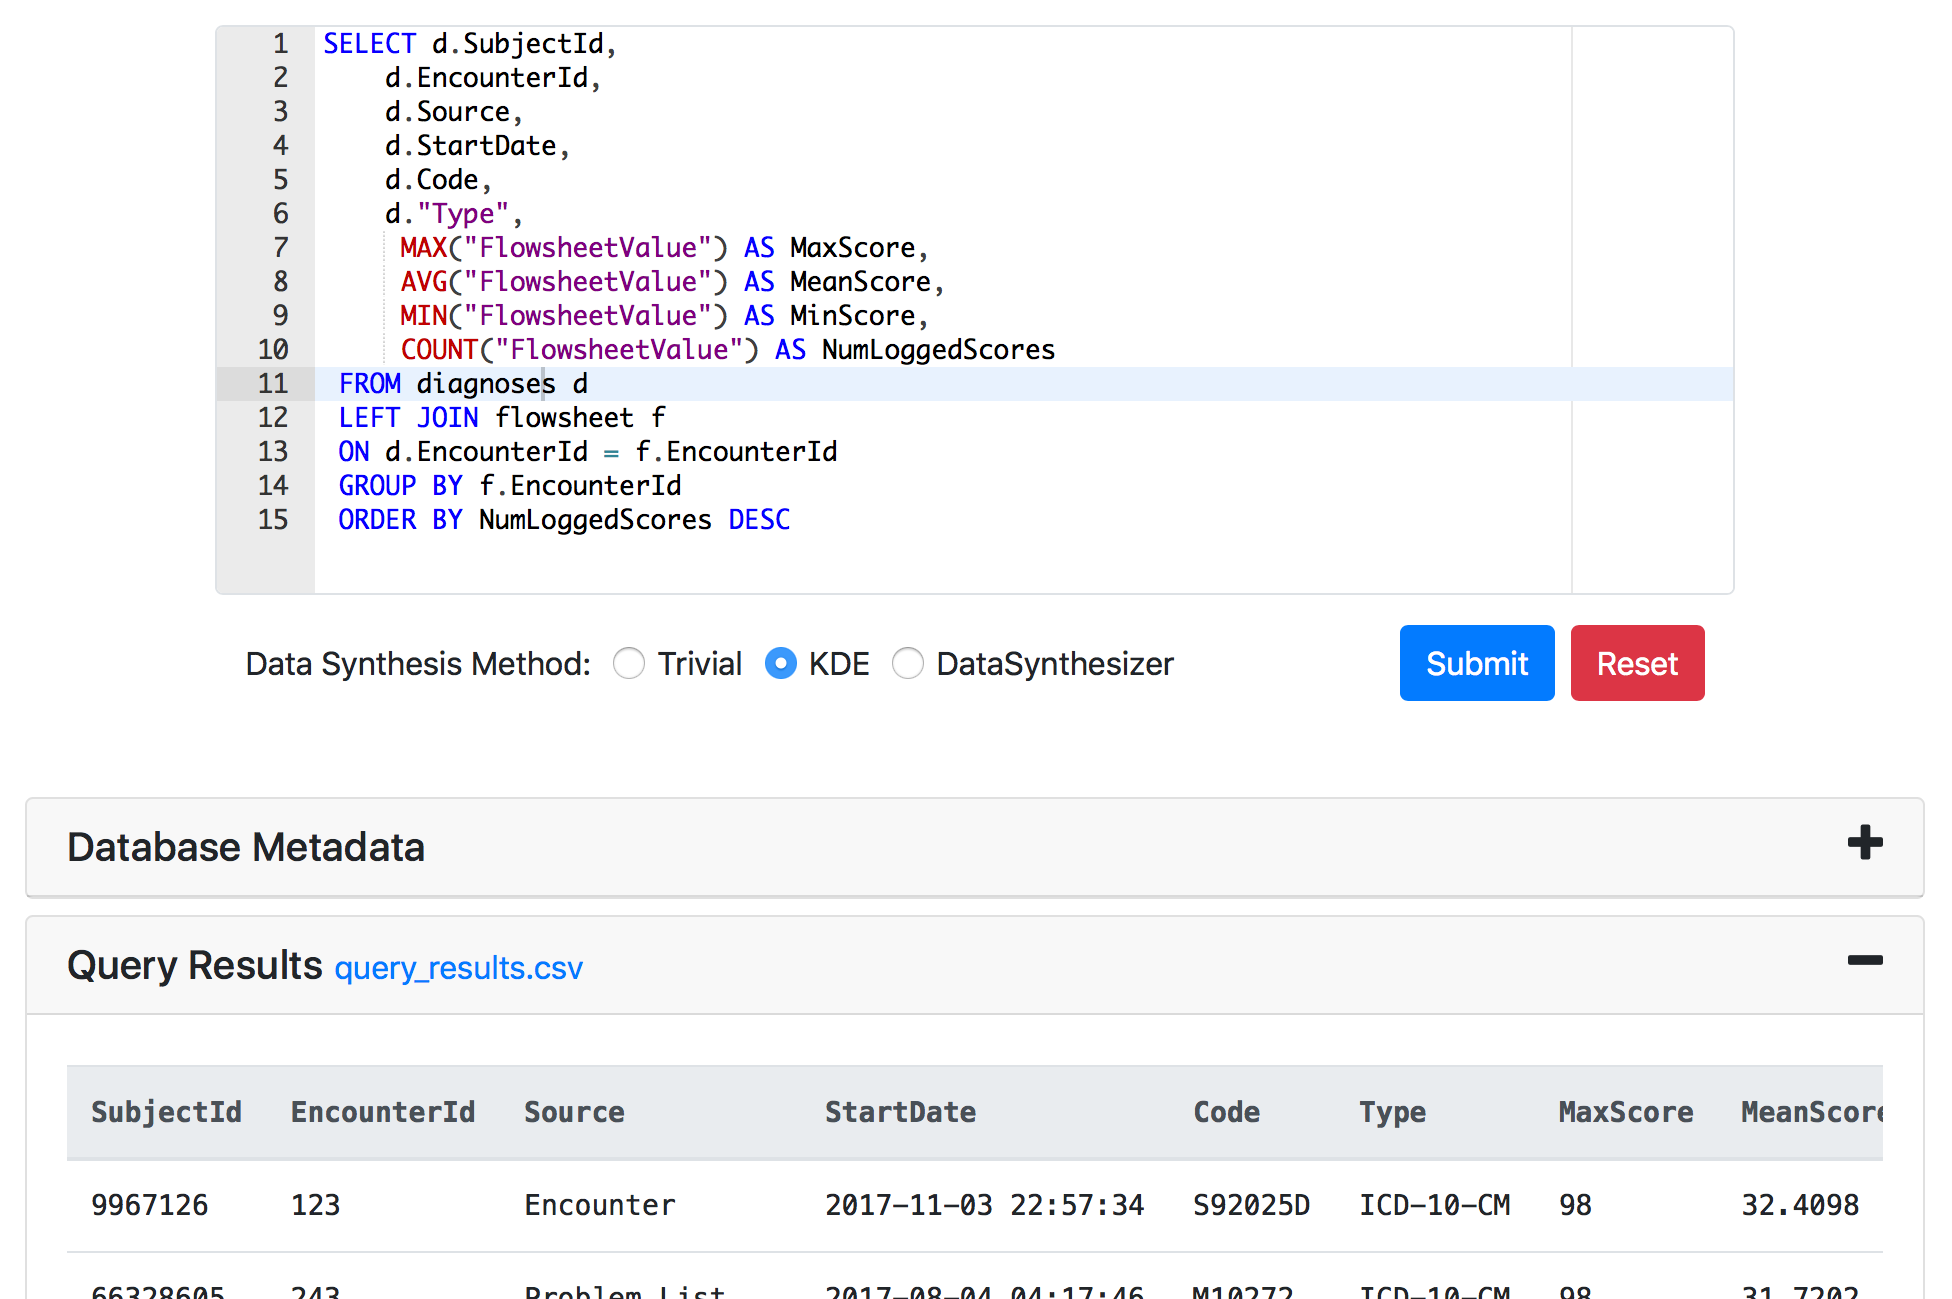
\includegraphics[width=0.5\textwidth]{ui_screenshot3}
  \caption{User Interface.}
  \label{fig:ui}
\end{wrapfigure}
